\chapter{Literature Review}
\label{chp:Literature Review}
This chapter aims to describe the biological context within which the project is undertaken. An overview of the anatomy of the ear, which is relevant to this study, is given. Thereafter, background is given of the physiology of each of the four vital signs. Finally, the technology relevant to the measurement of each vital sign required of the Ear-Monitor is discussed in terms of theory and the work done by others.

\section{Ear Anatomy} %----------------------------------------------------------------------------------
The area that is available for the Ear-Monitor to make the vital sign measurements is the external ear. It includes the auricle, ear canal with surrounding tissue and the lateral side of the tympanum.  Each part of the ear anatomy is discussed, especially with regards to its ability to emit information related to vital signs or to support the device in another way.

\subsection{Auricle}
The auricle is the visible part of the ear. It forms a C-shaped funnel that protrudes from the scull. Its structure is predominantly formed by yellow elastic cartilage covered in skin. Its complex folded shape differs from person to person, but certain structures are present in all normal auricles and have been named. As can be seen on Figure \ref{fig:Auricle}, the concha is the indented part next to the ear canal. This area is an ideal location for a wearable device. The device can be held in place by the tragus and a probe can easily extend into the ear canal.

\medskip

The external ear is supplied with blood from the auricular arteries. These arteries branch from the carotid artery which supplies the rest of the brain with blood. Being made mostly of cartilage and located at an extremity of the body, the auricle is not a suitable location for taking temperature measurements for its temperature is easily influenced by the ambient conditions.

\medskip

\begin{figure}[H]
\centering
\graphicspath{{figs/}}
\def\svgwidth{200pt}
\input{figs/Auricle.pdf_tex}
\caption{Anatomical structures of the auricle}
\label{fig:Auricle}
\end{figure}

The layer of skin covering the auricle contains blood vessels and therefore the earlobe is a popular location for traditional pulse oximetry measurements. This is a possible location for an ear-worn device to make a heart rate and peripheral blood oxygen saturation (SpO\textsubscript{2}) measurement \citep{poh2010motion}. The earlobe's blood vessels are, however, susceptible to vasoconstriction due to cold or hypovolaemia \citep{WHO2011UsingPulseOxi}. This will reduce the blood perfusion of the subcutaneous tissue making it harder to record accurate heart rate and SpO\textsubscript{2} measurements.

\subsection{Ear Canal}
The external ear canal is the tube running from the floor of the auricle to the middle ear, ending blindly at the tympanic membrane or tympanum. Figure~\ref{fig:EarSection} depicts the structure of the ear as seen from a coronal plane section. The auricle is visible and the shape and relative size of the canal can be observed.
The ear canal in adults is approximately 25 mm long and have a diameter of 5 to 7 mm \citep{alvord1997anatomy}. The outer third of the external ear canal is surrounded by cartilage and fibrous tissue \citep{ExternalAuditoryCanal}. The inner two thirds is surrounded by the temporal bone. Thin skin forms the lining of the canal and contains glands secreting ear wax. Hairs are found in the outer part of the canal. The ear canal of infants starts out relatively straight, but obtains a definite S-shape as the head develops \citep{alvord1997anatomy}. This S-shape is important to keep in mind when placing a sensor to measure tympanic temperature. Ear canal size also varies from person to person. Therefore, an ear probe should be designed to fit in a variety of ear canal shapes and sizes.

\begin{figure}
   \centering
   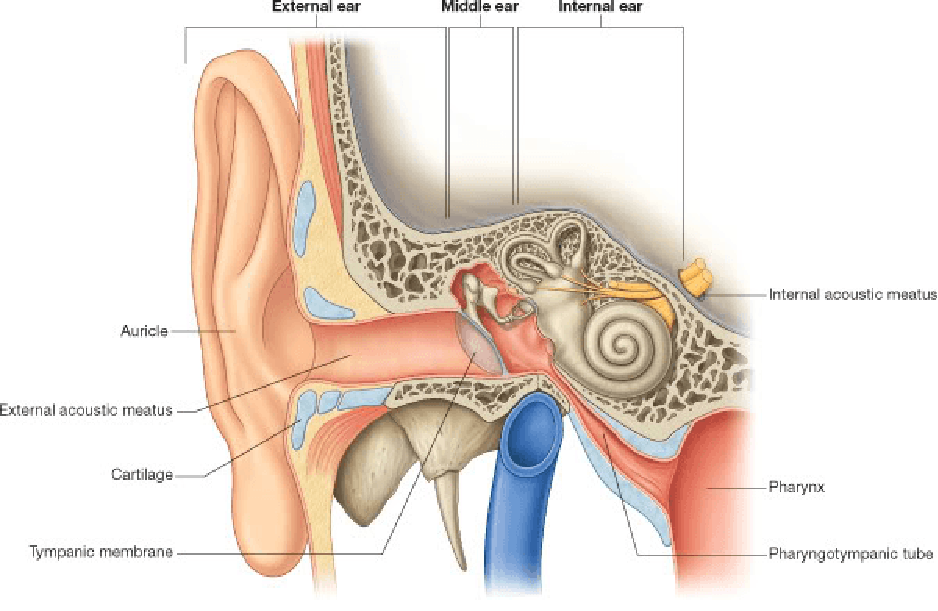
\includegraphics[scale=0.7]{figs/EarSection}
   \caption{Structure of the ear (Drake et al: Gray's Anatomy for Students)}
   \label{fig:EarSection}
\end{figure}

\medskip
The secluded nature of the ear canal means that it has a relatively constant temperature. Air trapped in the canal by a plug of high thermal resistance will reach thermal equilibrium close to the temperature of the canal wall and tympanum. This is a better location for a core temperature measurement, but will still be influenced by the ambient temperature.
The wall of the ear canal is well supplied with blood. Blood vessels just beneath the thin layer of skin make the ear canal a possible location for measuring heart rate and blood oxygen saturation. The still nature of the head will minimize movement artefacts.

%The ear canal extends towards the brain and electrical brain activity is present due to the conductive nature of the tissue. According to \cite{nunez2006electric} currents from brain potentials can be focused through holes in the scull, like the ear and nose. The further away the origin of the signal is from the electrode, the weaker the measured signal will be. Therefore, an electrode in the ear canal will detect electrical brain activity near the ear better, including the temporal lobe and brain stem.

\subsection{Tympanic Membrane}
The tympanum forms the medial boundary of the external ear canal. It is a smooth elliptical membrane with a thickness of about 0.074 mm \citep{alvord1997anatomy}. The membrane is slanted relative to the external ear canal.

\medskip
As with the rest of the external ear, the tympanum is supplied with blood from a branch of the carotid artery, therefore sharing its supply with the brain, including the hypothalamus, the thermoregulation centre of the body. It is the most medial part of the external ear, and is therefore the least susceptible to be influenced by the ambient temperature. This is the reason why the tympanum is one of the best locations to measure core body temperature. The location is used by physicians to measure core temperature, for it is quick and minimally invasive \citep{gasim2013accuracy}. Variations in body temperature can be sensed faster on the tympanic membrane than on other locations on the body. Contact with the tympanum can cause discomfort and harm to the patient, so non-contact infrared thermometers are usually used.


\section{Vital Sign Physiology} %----------------------------------------------------------------------------------
This section reviews the theory and research done on the physiological aspects of each vital sign that the Ear-Monitor is required to measure. The importance of each of the four vital signs are discussed, including the typical range of measurements expected from healthy adults and the causes and implications of deviations from these measurements.

\subsection{Core Temperature}
Thermoregulation is the body's way of keeping its internal temperature within certain limits to create a favourable environment for chemical reactions to take place \citep{thermoregulation2016}. The temperature control centre of the body is in the hypothalamus and it regulates temperature by maintaining a fine balance between heat production and heat loss. Normal human core temperature varies between \SI{36.5}{\celsius} and \SI{37.5}{\celsius} \citep{jones2010biomedical}. Inability to maintain this balance may indicate problems in the well-being of a person. Elevated temperature (hyperthermia) due to a fever can indicate the presence of an infectious disease. Abnormally low temperature (hypothermia) can be caused by exposure to cold, metabolic disorders or infection. Both hyper- and hypothermia can be life threatening. A core temperature measurement is often a key indication to start a treatment or not. Therefore, temperature measurement is part of a full clinical examination.

\medskip
The location where temperature is measured is a key factor, for temperature is not constant throughout the body. This is because heat production and heat loss are not constant throughout the body, which means extremities are usually cooler than the core. Traditional locations for measuring temperature are the tympanic membrane, axilla, mouth, rectum, oesophagus, forehead and urinary bladder. The mean temperature of these areas varies as well. A systematic literature review done by \cite{sund2002normal} combined the results of 20 studies to identify oral, rectal, tympanic and axillary temperature ranges in healthy humans. Figure \ref{fig:VariationsInTemp} illustrates the results.

 \begin{figure}
   \centering
   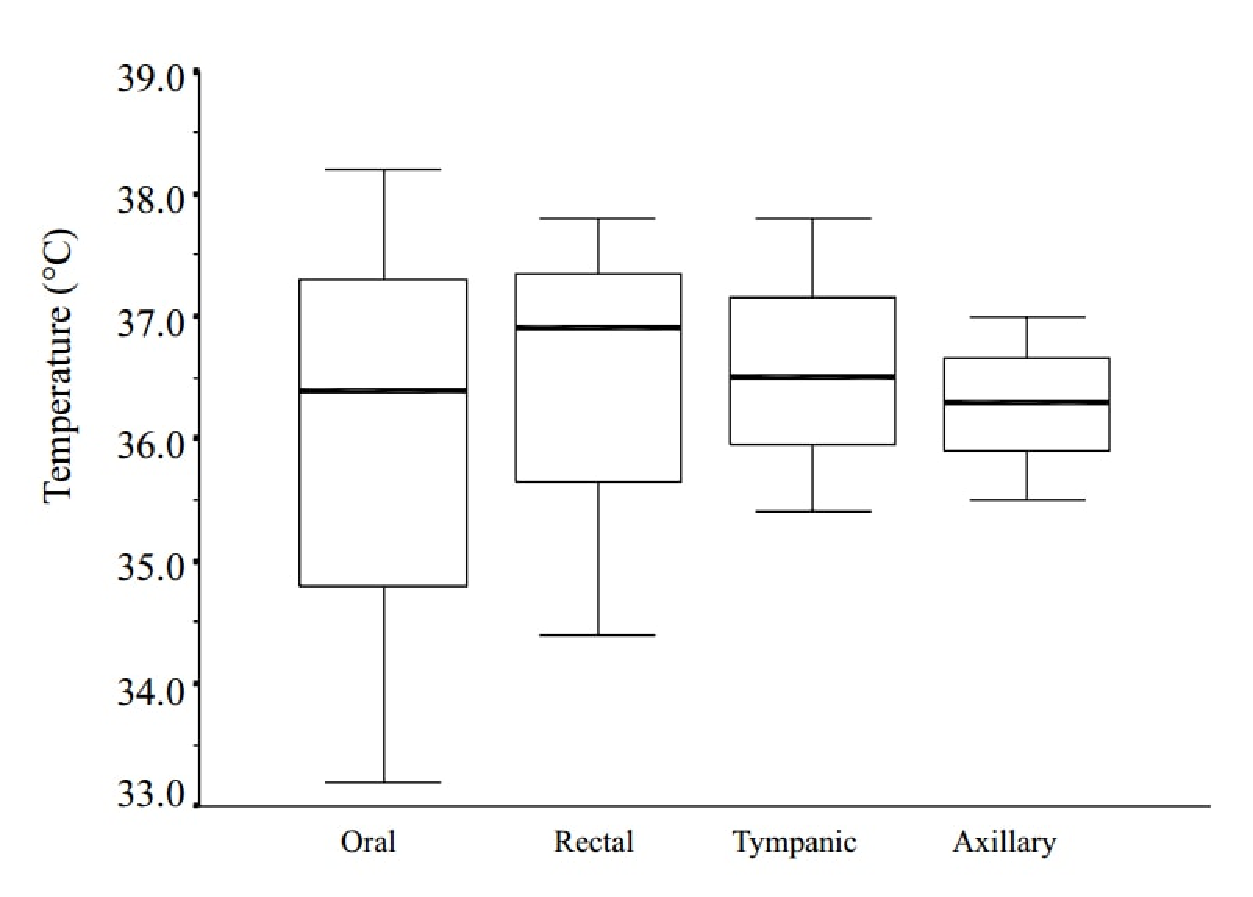
\includegraphics[scale=0.3]{figs/VariationsInTemp}
   \caption{The results from 20 studies reviewed by \cite{sund2002normal}}
   \label{fig:VariationsInTemp}
\end{figure}

\medskip
Studies have also been done comparing measurements at distinct locations to pulmonary artery temperature in ill patients. One of these found the following standard errors for temperatures at different locations: to ear-based  $0.07\pm \SI{0.41}{\celsius}$; urinary bladder  $0.03\pm \SI{0.23}{\celsius}$; oral  $0.05\pm \SI{0.26}{\celsius}$; and axillary $-0.68\pm \SI{0.57}{\celsius}$. The accuracy of each method varied with the level of pulmonary artery temperature. Repeated measurements with all four methods had mean standard deviation values within $\pm \SI{0.2}{\celsius}$ \citep{erickson1993comparison}.

\medskip
A second study done by \cite{lefrant2003temperature} showed the following standard errors: oesophageal  $0.11 \pm \SI{0.30}{\celsius}$, rectal $-0.07 \pm \SI{0.40}{\celsius}$, axillary $0.27\pm \SI{0.45}{\celsius}$, inguinal $0.17 \pm \SI{0.4}{\celsius}$ and urinary bladder $-0.21 \pm \SI{0.20}{\celsius}$.

\medskip
The location of the device in development is restricted to the ear, therefore the tympanic membrane is the preferred location for temperature measurements. The referenced studies show that the tympanic membrane is a valid location to measure accurate core temperature.

\subsection{Heart Rate}
The presence of a heart beat is paramount to sustain the vital cardiac output, supplying blood to the whole body. Heart rate can be controlled or maintained through two different regulatory systems: The intrinsic conduction system and the nervous system. The intrinsic conduction system works through the rhythmic contraction and relaxation of the heart muscle tissue. The heart rhythm is regulated by the sinoatrial node. The nervous system can influence the heart rate through sympathetic and parasympathetic nerves running from the cardiovascular centre in the medulla oblongata to the heart. The heart beat rate is varied to control the blood flow and blood pressure in the body.

\medskip
The heart is the source of a group of bio-signals. The firing of nodes and propagation of electrical charges through neurons and the conductive cardiac muscles emit electrical signals that can be detected. The contraction of the  ventricles forces blood into the arteries, causing a temporary increase in blood pressure. This pressure increase propagates through the arteries as a wave, causing a temporary local increase in blood volume. Pressure- and volume changes can be detected. Blood turbulence and the opening and closing of heart valves cause the characteristic heart sound and chest movements, both indications of heart rate.

\medskip
Heart rate is influenced by numerous physiological factors including $O_2$, $CO_2$, $H^+$ levels, blood pressure, stress and exercise. Pathological factors can include fever, sepsis, heart disease and anaemia. Tachycardia is abnormally high resting heart rate, generally above 100 bpm, whereas bradycardia is a lower than normal resting heart rate, usually below 60 beats per minute (bpm) \citep{normalRestingHR}. Although these two conditions are not necessarily danger signs, it may be an indication of health problems and therefore heart rate measurement is part of any medical examination.

\subsection{Respiratory Rate}
Respiration is the first step in the chain of events to get oxygen to the body's cells for metabolism to provide the body with energy. Respiration ventilates the lungs with air through inhalation and exhalation. The respiratory rate of a healthy adult at rest is usually between 12 and 20 breaths per minute \citep{medscapeBreathingRate}. This can vary drastically if the body is experiencing physical or emotional stress. An increase in respiratory rate can be caused by a fever, pulmonary dysfunction or any one of numerous medical conditions.

\medskip
Respiratory rate monitoring is especially useful for diagnosing sleep apnoea. Symptoms include regular pauses in respiration or periods of shallow breathing (hypopnea) during sleep. This causes an oxygen deficiency in the body and lowers the quality of sleep. Short term symptoms include excessive daytime sleepiness, morning headaches, impaired alertness, and vision problems. If left untreated, sleep apnoea can lead to high blood pressure, diabetes, depression, worsening of ADHD, stroke, heart failure, irregular heartbeats, and heart attacks \citep{webMDSleepApnoea}. Sufferers may be unaware of their condition and a sure-fire method of diagnosing it is by monitoring respiratory rate during sleep, traditionally done during an overnight sleep study.

\subsection{Blood Oxygen Saturation}

Haemoglobin is the oxygen transporter protein found in red blood cells of blood. Blood gets oxygenated in the lungs and then carries O\textsubscript{2} to the rest of the body for aerobic respiration necessary to produce energy. The correct levels of oxygen in the blood are vital to the health of the individual.

\medskip
Arterial oxygen saturation, SaO\textsubscript{2}, refers to the concentration fraction of oxygenated haemoglobin to total concentration of haemoglobin in arterial blood. This fraction can be calculated by Equation \ref{eq:SaO2}.
\begin{equation}
\label{eq:SaO2}
SaO_2  =  \frac{C(HbO_2)}{C(HbO_2)+C(Hb)}
\end{equation}
Where $C(HbO_2)$ is the concentration of deoxygenated haemoglobin (deoxyhaemoglobin) and $C(Hb)$ is the concentration of oxygenated haemoglobin (oxyhaemoglobin).

\medskip
Blood oxygen saturation of 95-100\% is normal in healthy humans. Hypoxaemia is the condition when the saturation is below 90\%. This can be an indication of circulatory or ventilatory problems, anaemia or sleep apnoea. Levels below 80\% can impede organ function and can lead to organ failure and cardiac- or respiratory arrest. The brain is extremely susceptible to damage when deprived of oxygen. Cerebral hypoxia is the insufficient supply of oxygen to the brain. This can cause brain damage and in severe cases, brain death.

%\subsection{Electrical Brain Activity}
%EEG, or electroencephalography, is the non invasive recording of the electrical activity in the brain over time. The neurons in the brain %conduct electrical current


%\cite{bickford1951electroencephalography}

%\begin{figure}[h]
%\centering
%\graphicspath{{figs/}}
%\def\svgwidth{300pt}
%\input{figs/eegRhythm.pdf_tex}
%\caption{EEG rhythms}
%\label{fig:eegRhythm}
%\end{figure}



\section{Vital Signs Measurement Theory}
This section will accumulate a thorough understanding of the theory and current state of technology relevant to the measurement of each vital sign required of the Ear-Monitor. Attention is given to the different methods available to determine each vital sign. This section will also make reference to various articles and studies done by other researchers in this field of study. The aim is to gather all the relevant information to make an informed selection of the methods and sensors the Ear-Monitor will use to measure each vital sign.

\subsection{Core Temperature Measurement}
Various methods are available for measuring core temperature. Non-electric, fluid-filled thermometers was the first to be used \citep{pearce2002brief}. The mercury-filled thermometer was used by early physicians to study the thermoregulation of the human body and crudely identify fevers. Since then, the mercury has been replaced by coloured alcohol or another heat sensitive liquid, due to toxicity of mercury.

\medskip
Another type of fluid-filled thermometer is the liquid-crystal thermometer. It contains liquid crystals that change colour at different temperatures. The use of these two types of fluid-filled thermometers has decreased significantly due to the accuracy, speed and convenience of digital thermometers.

\medskip
Digital thermometers are now the industry standard of measuring core temperature. Central to any digital thermometer lies a transducer that convert temperature to an electrical signal. Resistance temperature detectors, thermocouples thermistor and thermopiles are discussed. They can be divided into contact and non-contact thermometers.

\subsubsection{Contact Thermometers}
These are a family of thermometers that measure their own temperature with the assumption they and the object whose temperature is of interest, are in thermal equilibrium. Therefore, they are usually placed in contact with the object. When using a contact thermometer in the ear, the sensor part of the thermometer can be placed in contact with the ear canal wall, the air inside the canal or with the tympanic membrane itself. Several types of contact thermometers exist, including resistance temperature detectors, thermocouples and thermistors.

\begin{description}
\item[Resistance Temperature Detector] \hfill \\Resistance temperature detectors (RTDs) use the temperature-resistance relationship for metals to measure temperature. Thin wire coils or films of platinum, copper or nickel are usually preferred for they have a stable and repeatable temperature-resistance relationship over a wide temperature range.

\item[Thermocouple] \hfill \\
Thermocouples make use of the thermo-electric effect to make a temperature measurement. They consist of two dissimilar conductors connected at the one end, knows as the hot junction (measuring junction). The other ends of the two wires are known as the cold junction (reference junction) and are connected to a voltage meter via common conductors. A voltage is generated dependent on the temperature difference between the measuring- and reference junctions. Thermocouples do not respond to absolute temperature; therefore, their accuracy depends on how well the reference temperature can be defined. Reference temperatures are usually determined by a precise thermistor. Thermocouples are very versatile and widely used in clinical applications, but the downside is that their output signal is low and non-linear, therefore requiring a sensitive and stable voltage measuring device \citep{jones2010biomedical}.

\medskip
Thermocouples can be connected in series and are then called thermopiles. This configuration sums the output voltages, resulting in temperature averaging. This method improves accuracy by reducing noise. 

\item[Thermistor] \hfill \\
A thermistor is a type of semiconductor whose resistance varies with changes in temperature. They differ from RTDs in that they are usually made of ceramics, they have higher precision over a smaller temperature range and they can have a negative relation to temperature. Thermistors are preferred above RTDs and thermocouples for use as biomedical sensors due to their faster response time and higher sensitivity over a smaller range. The smaller range does not matter, for the temperature range of interest in bio-sensors is small and well defined.

\item[Contact Thermometer Application] \hfill \\
In the case of RTDs and thermistors, the measuring element is placed in position and a current is sent through the sensor. By measuring the voltage across the resistive element, it is possible to calculate the voltage and subsequently determine the temperature. In the case of a thermocouple, the hot junction can be placed in contact with the canal wall or tympanum. Typically, the hot junction is enclosed in a soft material to protect the canal and tympanum. The canal is sealed off and time is allowed for the area to equilibrate to tympanic temperature.

\medskip
Placing a thermometer in contact with the tympanic membrane gives an accurate measurement, but can cause discomfort to the wearer. There is also a risk of harming the tympanic membrane. Sensors in contact with the ear canal wall or the air inside the canal run the risk of making errors by measuring the temperature of objects that are not in thermal equilibrium with the tympanic membrane. Therefore, non-contact thermometers are considered.
\end{description}


\subsubsection{Non-contact Thermometers}
Thermopiles can be used to detect thermal radiation without being in contact with the object. All matter with temperatures above 0 K radiates electromagnetic radiation according to the Stefan-Boltzman law. The thermal radiation, $Q$, per unit area is given by Equation \ref{eq:Stefan-Boltzman}.
\begin{equation}
\label{eq:Stefan-Boltzman}
Q=\varepsilon \sigma T^4
\end{equation}

Where $\varepsilon$ is the emissivity, $\sigma$ the Stefan-Boltzman constant and $T$ the temperature of the object.
The wavelength distribution varies according to the temperature of the object and is described by Planck's law, given by Equation \ref{eq:PlancksLaw}.
\begin{equation}
\label{eq:PlancksLaw}
B_\lambda (\lambda ,T)=\frac{2hc^2}{\lambda ^5}\frac{1}{e^\frac{hc}{\lambda k_B T} -1}
\end{equation}

Where $B_\lambda$ is the spectral radiance, $\lambda$ the radiation wavelength, $h$ Planck's constant, $k_B$ Boltzman's constant $c$ the speed of light and $T$ the temperature of the object. By maximizing $B_\lambda$, it is possible to find the dominant wavelength that is emitted at a certain temperature. Figure \ref{fig:PlancksLaw} depicts a plot made of spectral radiance versus wavelength at $T=\SI{37}{\celsius}$, the core temperature of humans. It is evident that the dominant wavelength is at \SI{9.35}{\micro\meter}. This is in the infrared range, and therefore this type of thermal radiation thermometer is called an infrared thermometer.

\medskip

\begin{figure}[h]
   \centering
   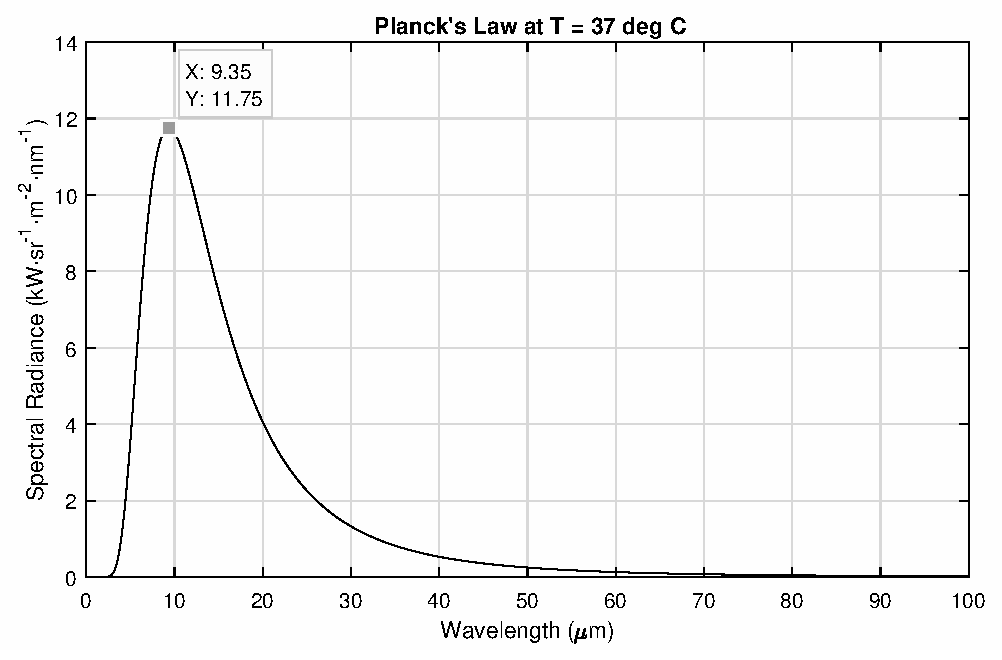
\includegraphics[scale=0.6]{figs/PlancksLaw}
   \caption{Dominant radiation wavelength at \SI{37}{\celsius} using Planck's law}
   \label{fig:PlancksLaw}
\end{figure}

In the case of measuring the temperature of the tympanic membrane, the temperature of the hot junction is determined by the radiation received from the tympanum minus the radiation radiated by the sensor itself.

\medskip

When dealing with thermal radiation, an important aspect is emissivity. Emissivity is the ability of an object to radiate thermal energy. It is quantified as a ratio of thermal energy emitted by a surface relative to the thermal energy emitted by an ideal blackbody at the same temperature. A blackbody has an idealized surface that reflects no radiation, which means all energy radiated from the surface is due to the temperature of the surface. Thus, a blackbody has an emissivity of 1 and has the maximum theoretical thermal radiation at a given temperature. The accuracy of an infrared sensor depends on the ability of the object to emit sufficient thermal radiation for the sensor to detect. Cross-referencing various emissivity tables, it was found that the emissivity of human skin is 0.98, which means that it is an excellent emitter of thermal energy \citep{stumme2003emissivity, EmissivityThermoWorks, EmissivityOptotherm}. The ear drum is covered with skin, making it an ideal target object for a non-contact thermometer.

\medskip

An infrared thermometer generally consists of a thermophile attached to a blackbody and shielded by an infrared filter that also acts as a lens to focus infrared waves \citep{irTempSensors}. This setup, depicted in Figure \ref{fig:IR_Thermometer}, allows for the non-contact temperature sensing of the tympanic membrane. Unlike pulse and respiratory rates, core body temperature varies slowly. It takes minutes to vary significantly. Therefore, the sampling period of core temperature can be as long as 10 seconds.

\medskip

\begin{figure}
   \centering
   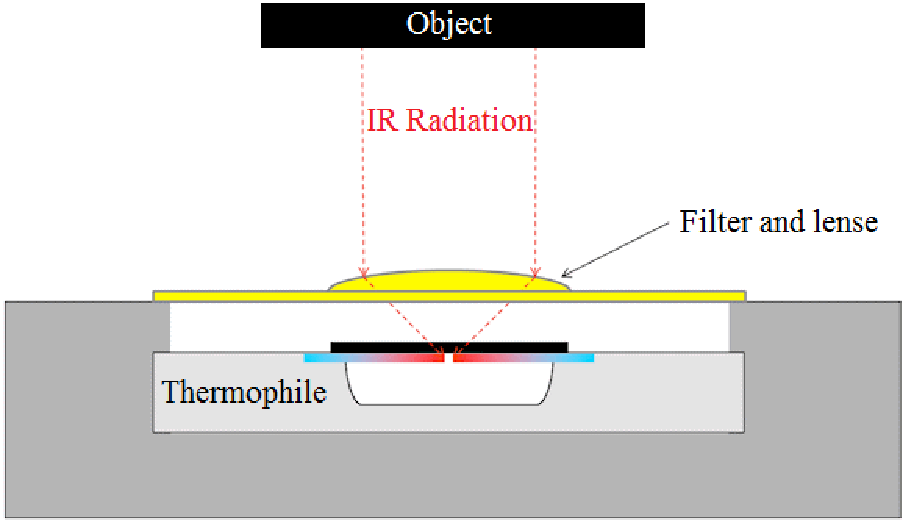
\includegraphics[scale=0.5]{figs/IR_Thermometer}
   \caption{Infrared thermometer diagram \citep{irTempSensors}}
   \label{fig:IR_Thermometer}
\end{figure}

\subsection{Commercial Temperature Monitoring Devices}
Ear thermometers are widely used at home and in hospitals. Ear contact thermometers like Novatemp\textsuperscript \textregistered{} and Starboard\textsuperscript \textregistered{} claim a $\pm\SI{0.2}{\celsius}$ accuracy \citep{Novatemp, Starboard}. Non-contact infrared ear thermometers usually have a similar rated accuracy. None of these are, however, wearable devices. 

\medskip
 
The Degree\textsuperscript \textregistered{}, Figure \ref{fig:Degree}, is a continuous in-ear thermometer for children, developed by Cosinuss, a company specialising in wearable sensors. The bulk of the device is worn behind the ear, and a wire runs over the auricle to the ear canal, in which a probe is placed. The device takes its temperature measurements with a sensor placed in contact with the canal wall. The manufacturer claims an accuracy of $\pm\SI{0.1}{\celsius}$ \citep{CosinussDegree}. It monitors temperature continuously and sends real time data to a mobile phone.

\medskip

\begin{figure}[h]
   \centering
   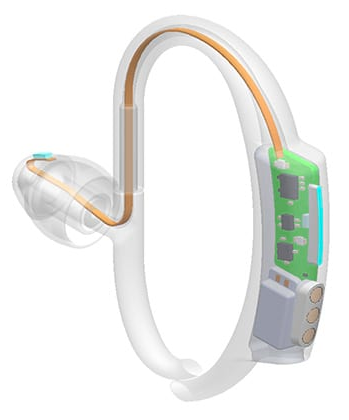
\includegraphics[scale=0.5]{figs/Degree}
   \caption{CAD model of the Degree from the Cusinuss website \citep{CosinussDegree}}
   \label{fig:Degree}
\end{figure}

Apart from the Degree, there is not much literature on wearable ear thermometers. Two patents were found describing similar devices: US 6556852 B1 and US 20090221888 A1. The first proposes the use of an infrared sensor pointed at the tympanic membrane, and the latter does not specify the method of measuring. The trial planned as part of this project will add to this insufficient body of knowledge.

\section{Heart Rate}
%The heart is a very dynamic organ whose influence can be felt throughout the body.
There are many options available to monitor heart rate. Electronic monitoring methods include electrocardiography, photoplethysmography, ballistocardiography, phonocardiography and doppler flow-meters.

\subsection{Electrocardiography}
Electrocardiography (ECG) is a recording of the electrical activity of the heart over a period of time. Electrical activity arises from the depolarization and repolarization of the heart muscle during the cardiac cycle. The most prominent electrical charge is the QRS complex, which corresponds to the ventricular depolarization and is visible on the electrocardiogram as a sharp peak in the millivolt range. ECG is the recommended way of monitoring heart rate in most intensive care units. A cardiologist will use a 12 lead ECG with 10 electrodes placed in a specific configuration on the chest. Various wearable devices use ECG to measure heart rate. Fitness monitors normally use a chest strap with electrodes to detect the electrical activity of the heart.

\medskip
Studies have been done developing wearable ECG devices for clinical use. The latest in wearable ECG electrodes is the use of dry polymer-based materials \citep{wang2010wearable} or non-contact electrodes that can be place on top of clothing \citep{lin2013development}. This is an improvement on the standard conductive gels or adhesives and can be used repeatedly. But these electrodes still need to be placed on the chest.

\medskip
An ear located ECG monitor has been developed by \cite{winokur2012wearable}. This device uses a single lead setup with one electrode placed on the mastoid bone behind the ear and a reference electrode placed on the neck. This configuration relies on the conductive properties of human tissue to carry electrical charges from the heart to the ear. They were able to use the electrocardiogram in conjunction with PPG and BCG to determine various heart intervals and track changes in mean arterial blood pressure. Figure \ref{fig:Winokur} depicts \cite{winokur2012wearable}'s device and a plot of its electrocardiogram. No heart rate information was extracted.

\medskip

\begin{figure}[H]
   \centering
   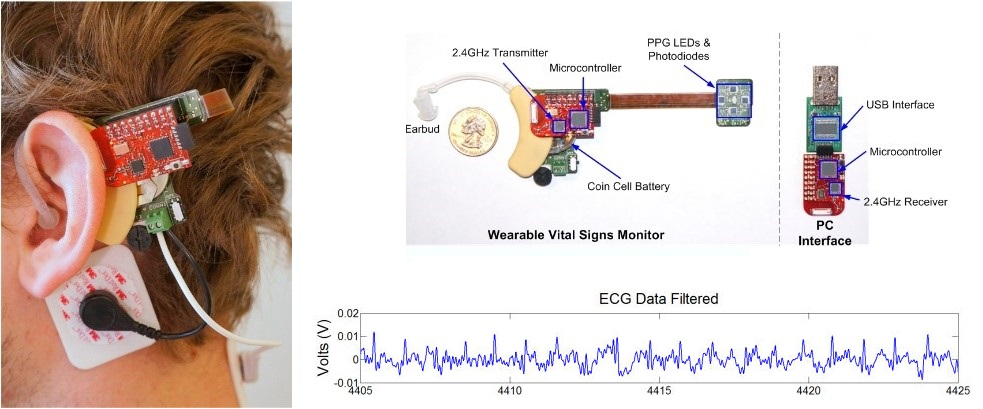
\includegraphics[scale=1.1]{figs/Winokur}
   \caption{Ear-worn device developed by \cite{winokur2012wearable}}
   \label{fig:Winokur}
\end{figure}

\subsection{Photoplethysmography}
Photoplethysmography (PPG) produces an optically obtained plethysmogram, which plots the volume of an organ over time. PPG can be used to measure the change in the volume of blood vessels close to the skin surface. When the left ventricle contracts a pressure pulse propagates through the arteries from the heart to the extremities of the body. This wave corresponds to the systolic blood pressure. Blood vessel walls contain elastic fibres that allow it to stretch. This means that the diameter of vessels will increase when the blood pressure increases, causing arteries to stretch and contract with each cardiac cycle. PPG can be used to determine heart rate by measuring this volumetric variation.

\medskip
A photoplethysmograph can non-invasively determine peripheral arterial blood volume by shining light through the skin surface, into the dermis and subcutaneous tissue and collecting the light transmitted or reflected. Light shined into the tissue can either be reflected, absorbed or allowed to transmit through. This leads to the two modes of PPG operation depicted by Figure \ref{fig:PPGModes}.

\medskip
 
\begin{figure}[h]
\centering
\graphicspath{{figs/}}
\input{figs/PPGModes.pdf_tex}
\caption{The two modes of Photoplethysmography \citep{tamura2014wearable}}
\label{fig:PPGModes}
\end{figure}

In (a) the emitter and detector face each other and are separated by tissue that can transmit the light, leading to a transmission mode PPG. Transmission mode PPG is limited to locations on the body where transmitted light can be detected, like the finger, ear lobe, concha and tragus. These locations have limited blood profusion, especially at low temperatures. In (b) the emitter and detector are placed on the same plane and both faces towards the tissue. Light from the emitter is reflected by the tissue and captured by the detector, leading the reflection mode PPG. The emitter and detector need to be optically isolated so that light cannot pass from the one to the other without going through the tissue. Reflectance mode PPG can be used at more locations, but is more susceptible to motion artefacts \citep{tamura2014wearable}.

\medskip
According to Lambert's law, the amount of light absorbed is proportional to the length of the path that the light has to travel in the absorbing substance \citep{lambertANDbeer}. Therefore, a change in blood vessel diameter will increase the distance the light has to travel causing a change in light absorption. This can be detected by measuring reflected or transmitted light. Variation in the light reflected or transmitted is synchronised with the heart rate.

\medskip
Shorter light wavelengths are mostly absorbed by the tissue, while longer wavelengths can penetrate deeper. Red and near infrared light are preferred for transmission PPG. Green light is becoming more popular for shallow reflectance PPG, due to larger light variations during the cardiac cycle and less noise than near infrared PPG \citep{tamura2014wearable}.

\medskip
The signal read by the photo detector of the pulse oximeter consists of an AC component superimposed on a DC signal. The DC component is due to the constant transmission or reflection of light by the body's tissue: skin, fat, venous blood and the non-pulsating arterial blood. The AC component is the variation in transmitted or reflected light due to the change in diameter of the arteries and therefore synchronised to the heart rate. The AC component is usually between 0.5 - 2\% of the DC component \citep{tavakoli2006analog}. Figure \ref{fig:PPG} illustrates the way in which the heart rate is visible in a photoplethysmograph. It can be seen that the blood volume increases with each heartbeat, and that this causes more light to be absorbed, thus less detected by the photodiode.

\medskip

\begin{figure}[h]
   \centering
   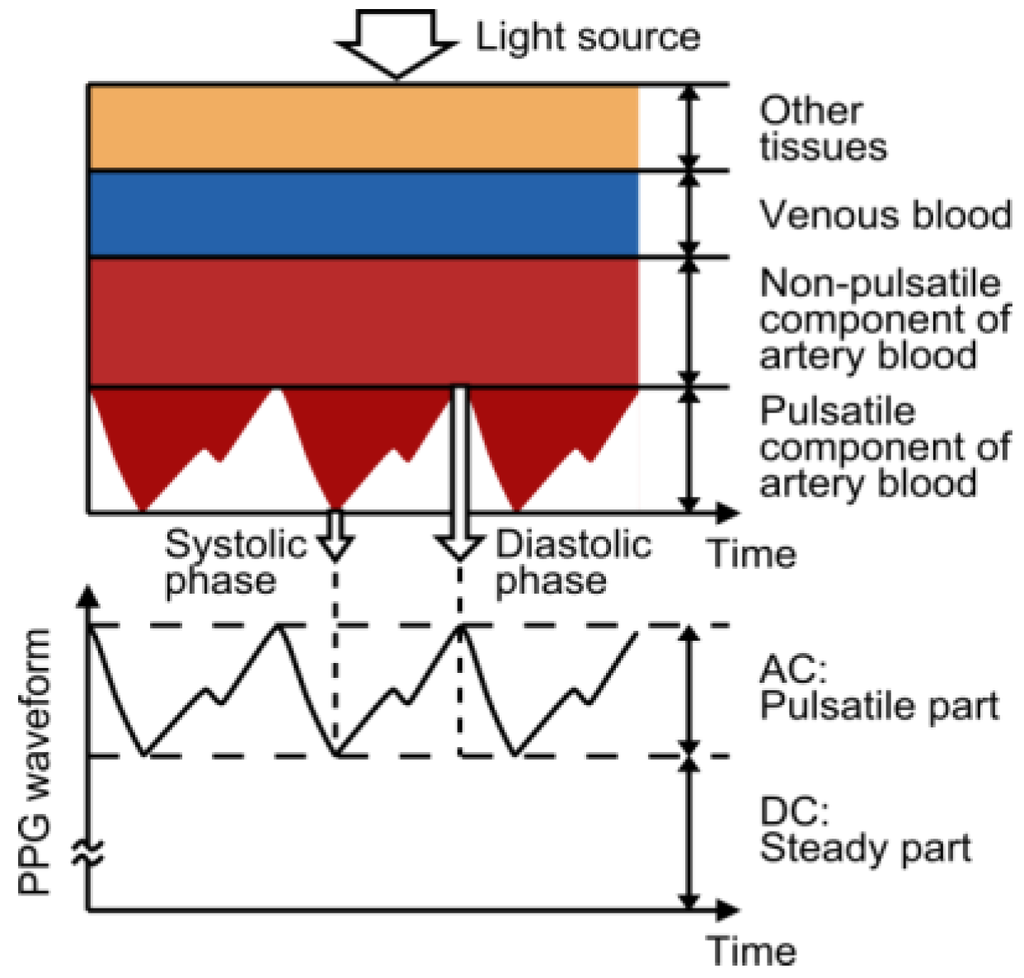
\includegraphics[scale=1.6]{figs/PPG}
   \caption{Basic operating principles of PPG \citep{tamura2014wearable}}
   \label{fig:PPG}
\end{figure}

\subsubsection{Work done by others in Ear PPG}
A review of work done by others in the field of ear PPG reveals six devices relevant to this study.

\medskip
\cite{shin2009novel} present a wearable music headset with an integrated transmission PPG ear clip that attaches to the ear lobe. The device includes an accelerometer to aid in the removal of motion artefacts. Evaluation was done through a study comparing the heart rate from the device to that made with a conventional ECG recorder. This study revealed a heart rate error of 0.6\%.

\medskip
\cite{poh2010motion} designed a wearable PPG with a magnetic earring sensor. The bulk of device sits in front of the ear and is held in place by a band around the auricle, as can be seen from Figure \ref{fig:poh}. A reflective PPG sensor is held against the ear lobe by placing a magnet on the opposite side. The device also includes an accelerometer to make baseline measurements for motion artefact cancellation. A study was conducted to compare the PPG signals measured by the wearable device to chest ECG signals collected by a FDA-approved commercial system. Whilst standing motionless, the study found a very high correlation between the ear PPG and the chest ECG with a mean bias of 0.62 $\pm$ 4.51\% with ECG reference measurements.

\medskip

\begin{figure}[h]
   \centering
   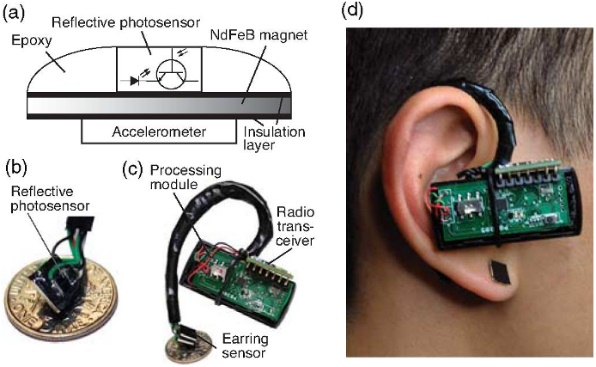
\includegraphics[scale=1.2]{figs/poh}
   \caption{Wearable ear PPG device by \cite{poh2010motion}}
   \label{fig:poh}
\end{figure}

\cite{da2010ear} researched an ear worn heart rate monitor containing a PPG sensor in reflectance mode. Red light is shined into the tissue behind the ear and collected by a photodiode chip with an integrated transimpedance amplifier. Signals were not digitalised on the device, but recorded and processed on MATLAB. The collected signal was compared with a transition finger PPG and a chest ECG. Figure \ref{fig:DaHe} illustrates this comparison.

\medskip

\begin{figure}[h]
   \centering
   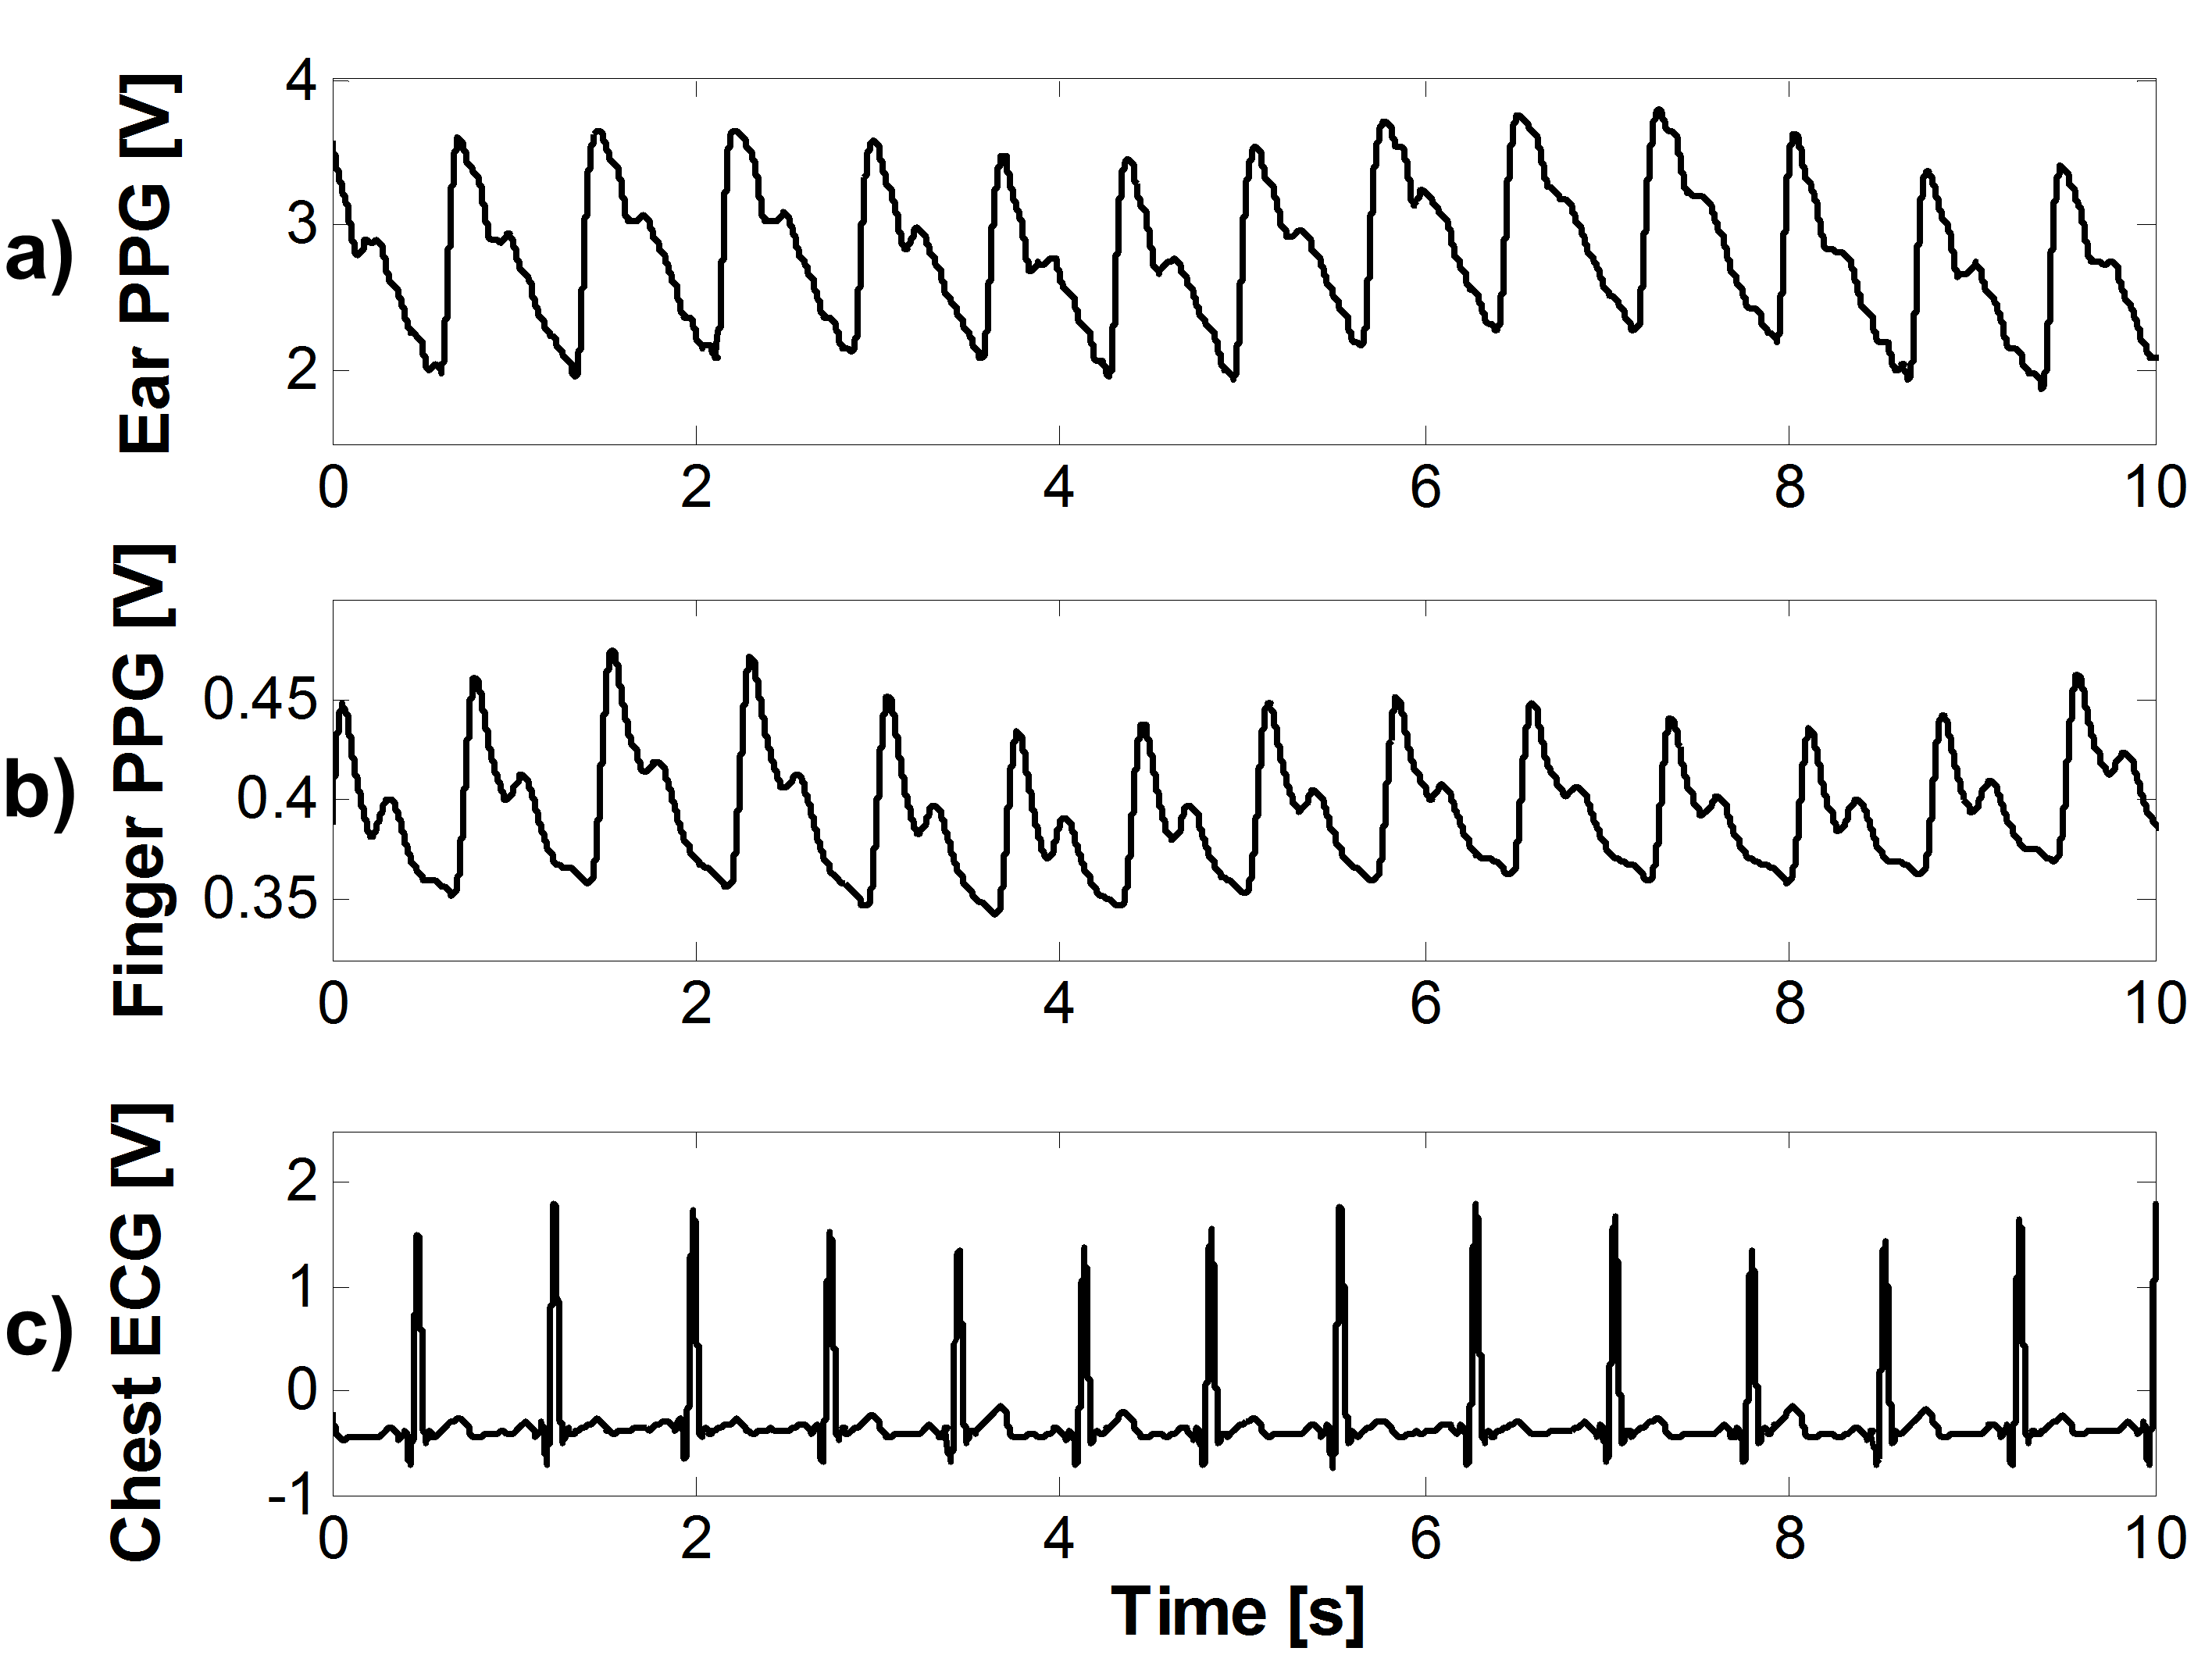
\includegraphics[scale=0.15]{figs/DaHe}
   \caption{Comparing ear PPG to finger PPG and chest ECG \citep{da2010ear}}
   \label{fig:DaHe}
\end{figure}

\cite{winokur2012wearable} developed a similar device that shines 660nm and 940nm light waves through tissue at the mastoid bone and collecting the reflected light with 4 photodetectors. A PPG front end conditioned the signals and their device sent the raw heart beat information to a PC through a radio connection. This is the same device that records ECG and is used to analyse heart intervals and mean blood pressure rather than heart rate.

\medskip
\cite{buskeheartbeat} proposed yet another location. They modified a pair of headphones to measure a transmission PPG from the concha. During the testing phase, the device showed a mean heart rate accuracy of around 85\% when compared to an ECG.

\medskip
The Cosinuss One\textsuperscript \textregistered{} is a commercial device that monitors heart rate through the ear canal. The earpiece presses against the ear canal wall and records a PPG in reflection mode. It targets athletes that want to monitor their bodies during exercise.

\begin{figure}[h]
   \centering
   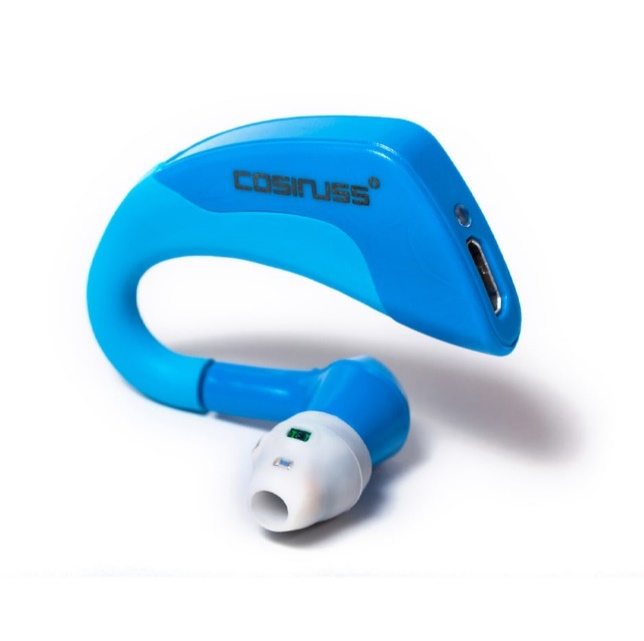
\includegraphics[scale=0.8]{figs/cosinuss}
   \caption{Cosinuss One\textsuperscript \textregistered{} ear worn heard rate device \citep{CosinussOne}}
   \label{fig:cosinuss}
\end{figure}


\subsection{Ballistocardiography}
Ballistocardiography (BCG) is the measurement of the mechanical effects of the beating heart on the body over time. Typically, accelerometers or pressure sensors are used to measure movement or forces on the surface of the body. BCG has been researched for use in ear heart rate extraction.

\medskip
In a wearable device proposed by \cite{da2010ear}, mechanical vibrations associated with heart rate are converted to electronic signals through capacitive sensing electrodes placed behind the ear. This method works by measuring the change in capacitance between the two electrodes as the distance between them changes due to heart rate vibrations.

\medskip
A study by \cite{winokur2012wearable} proposed measuring the head-to-foot axis recoil due to the blood-volume shift during cardiac ejection. This is done by placing a MEMS accelerometer behind the auricle. Due to the movement dependent method of operation this technology is extremely susceptible to motion artefacts and it can only be used when the body is stationary.

\medskip
A variation of this technology is discussed in an article by \cite{park2015wearable}. They propose using a scissor shaped hinge mechanism in the ear canal that measures the change in the canal size due to the in-ear blood pulse waves. The mechanical movement is converted to an electrical signal through a piezoelectric film sensor. Figure \ref{fig:BCGsensor} shows a drawing of this device from Park's 2015 article.

\begin{figure}[h]
   \centering
   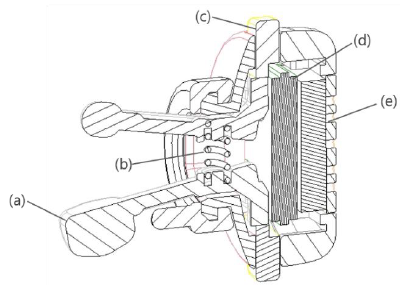
\includegraphics[scale=0.8]{figs/BCGsensor}
   \caption{Device to measure in ear pulse waves due to the heart beat \citep{park2015wearable}}
   \label{fig:BCGsensor}
\end{figure}

\subsection{Other Heart Rate Methods}
Electronic stethoscopes use a microphone to record heart sounds. The heat makes a distinct series of sounds during the cardiac cycle due to blood turbulence and the shutting of heart valves. A plot of the heart sounds is known as a phonocardiogram. The period of this sound series can be used to determine heart rate and it does not require skin-contact.

\medskip
A Doppler flow-meter can be used to detect the alternating blood current component in near-surface arteries. This component is synchronised to the heart rate frequency. The device can use ultrasound or electromagnetic waves to achieve the Doppler shift.

\medskip
A study done at Stanfort Medicine by \cite{shcherbina2017accuracy} reviewed seven commercially available wearable (wristband) heart rate monitors. They found mean errors ranging from 2.5 to 8.8\%.

\section{Respiratory Rate}
Unlike the other vital signs, a person cannot measure his or her own respiratory rate. As soon as a person is consciously thinking about respiration, breathing usually slows. Measuring needs to happen while the person's thoughts are otherwise occupied. Therefore, a continuous measuring method is preferred. Typically, a nasal mask or chest strap is used to measure respiration. 

\subsection{Respiratory Rate Ear Sensors}
Ear located devices that extract respiration information are rare, but some literature sources are available.

\medskip
\cite{goverdovsky2016hearables} tested an ear probe with two embedded microphones. The microphones could detect the sound created by turbulence in the airways for breathing rates higher than 12 breaths per minute. Figure \ref{fig:BreathingSound} shows a plot of the normalised sound amplitude at two different breathing rates. Variation during breathing can be seen in both recordings.

\begin{figure}[h]
   \centering
   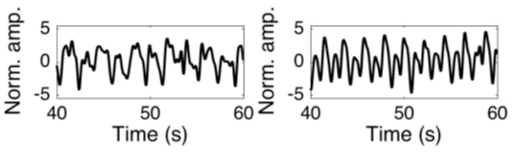
\includegraphics[scale=0.8]{figs/BreathingSound}
   \caption{Breathing detected through microphones inside the ear canal \citep{goverdovsky2016hearables}}
   \label{fig:BreathingSound}
\end{figure}

\cite{da2010ear} did extensive research on the ear as a location for vital sign monitoring. They extracted respiratory rate from baseline oscillations in a BCG signal recorded by capacitive electrodes placed behind the ear. Mechanical movement is converted to electrical signals by these electrodes. Therefore, the movement of the head due to respiration is seen on the BCG as baseline oscillations, Figure \ref{fig:BCGbreathing}.

\begin{figure}[h]
   \centering
   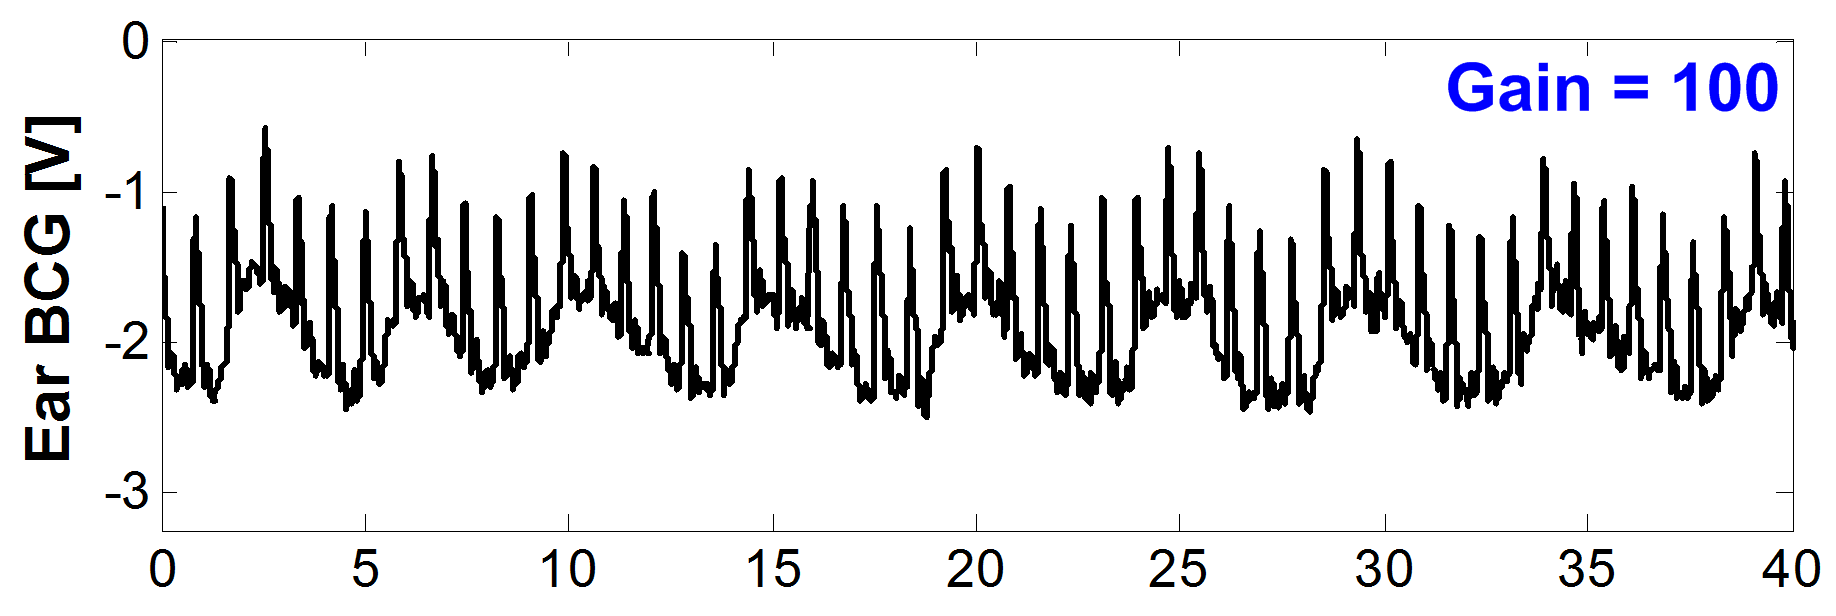
\includegraphics[scale=0.3]{figs/BCGbreathing}
   \caption{Baseline oscillations in behind the ear BCG due to breathing \citep{da2010ear}}
   \label{fig:BCGbreathing}
\end{figure}

\subsection{Respiratory related Heart Rate Characteristics}
A different approach is to extract respiratory rate by analysing the heart rate. A PPG signal contains three distinct respiratory related characteristics: amplitude modulation (AM), respiratory-induced intensity variation (RIIV) and frequency modulation \citep{johansson2003neural}.

\medskip
Amplitude modulation is due to blood pressure changes during the respiratory cycle called Pulsus Paradoxus. RIIV is changes in the volume of the dermis and subcutaneous capillary bed. It is visible as baseline variation in the PPG signal.  Frequency modulation of the heart rate synchronised to respiration rate, called respiratory sinus arrhythmia (RSA).

\medskip
RSA can also be detected in ECG, but differs from the fluctuations seen in chest ECG, due to electrodes movement relative to the heart and changes in chest impedance during the respiratory cycle \citep{moody1986clinical}. These fluctuations cannot be detected in the ear. RSA is observed as baseline oscillation in heart rate in synchrony with the respiratory rate. Heart rate increases during inspiration and decreases during expiration \citep{yasuma2004_RSA}. According to a study done by \cite{stratton2003effects}, the variation in heart rate due to RSA is higher in younger test subjects, with a 74\% increase in children versus a 52\% increase in adults.

\medskip
Research has been done to develop algorithms to utilise these characteristics to extract respiratory rate from PPG signals. \cite{clifton2007measurement} used wavelet analysis and achieved a respiratory rate accurate to within 1 breath per minute and \cite{leonard2006fully} documented a respiratory rate error of 7.9\%. \cite{johansson2003neural} developed two neural network algorithms that use the different respiratory related characteristics of PPG signals to detect breaths. Table \ref{table:RRC} shows the results of the best algorithm.

\begin{table}[H]
\centering
\caption{Results of the respiratory rate extraction through neural networks \citep{johansson2003neural}}
\begin{tabular}{P{5cm}P{3cm}P{3cm}}
 \hline
 Respiratory Related Characteristics & False Positive (\%) & False Negative (\%) \\ 
 \hline
 RSA  	& 	3.7 	& 	6.9 \\  
 AM 	& 	5.2 	& 	4.7 \\
 RIIV 	&	5.2		&	5.9 \\
 \hline
\end{tabular}
\label{table:RRC}
\end{table}


\section{Blood Oxygen Saturation}
Oxygen saturation can be measured by means of an arterial blood gas test resulting in an arterial oxygen saturation reading. This requires drawing a blood sample for testing and therefore is not relevant to this study. An alternative method is pulse oximetry. This method estimates peripheral capillary oxygen saturation, SpO\textsubscript{2}, through the spectrophotometric analysis of PPG signals captured at two different wavelengths. This is a clinically accepted estimation of the arterial oxygen saturation \citep{aoyagi2003pulse}.

\subsection{Pulse Oximetry Theory}
Blood oxygen saturation estimation through pulse oximetry relies on the different adsorption spectra of oxyhaemoglobin and deoxyhaemoglobin. Figure \ref{fig:AbsorptionSpectra} shows the absorption spectra of oxy- and deoxyhaemoglobin. 

\medskip
\begin{figure}[H]
   \centering
   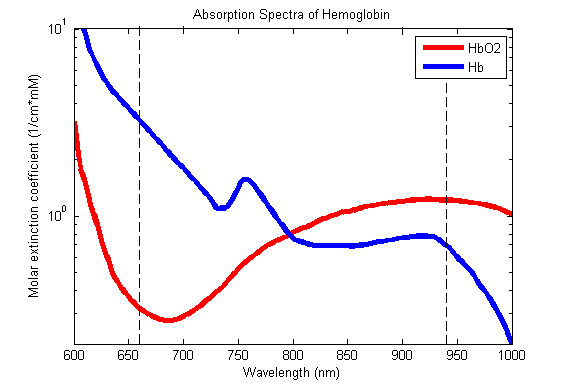
\includegraphics[scale=0.8]{figs/AbsorptionSpectra_Edit}
   \caption{Absorption spectra of oxy- and deoxyhemoglobin}
   \label{fig:AbsorptionSpectra}
\end{figure}

It can be noted that deoxyhaemoglobin has a significantly higher absorption of red light while oxyhaemoglobin has a slightly higher absorption of infrared light.

\medskip
According to Beers law, the amount of light absorbed by a dissolved substance is proportional to its concentration \citep{lambertANDbeer}. Therefore, oxygenated blood (with a higher concentration of oxyhaemoglobin) will absorb more infrared light and reflect more red light. Whereas deoxygenated blood (with a higher concentration of deoxyhaemoglobin) will absorb more red light and reflect more infrared light. This explains why oxygenated blood appears bright red, while deoxygenated blood is a darker shade of red.

\medskip
Red and infrared light are shined into the peripheral tissue and the light reflected or transmitted is measured for both wavelengths. Literature and commercial devices usually use wavelengths of 660 nm (red) and 940 nm (near infrared) \citep{tytler1986nellcor, ti2012datasheet, bagha2011real, bheema2013spo2, duun2007novel}. The ratio of reflected or transmitted light is unique to a certain level of blood oxygen saturation and is used to estimate blood oxygen saturation.

\medskip
The Beer-Lambert law describes the absorption of a specific wavelength of light by a substance in a homogeneous solution \citep{bagha2011real}. It can be used to calculate light intensity as show by Equation \ref{eq:BeerLambert1} or it can be manipulated to give what is called the unscattered absorption factor as shown in Equation \ref{eq:BeerLambert2} \citep{kennedy2015introduction}.
\begin{equation}
\label{eq:BeerLambert2}
I=I_o e^{-\varepsilon _\lambda cL}
\end{equation}
\begin{equation}
\label{eq:BeerLambert1}
A=\varepsilon cL=ln\left( \frac{I_o}{I}\right)
\end{equation}

\medskip
$A$ is the dimensionless adsorption factor, $\varepsilon$ is the wavelength dependant molar absorptivity, $c$ is the concentration of the substance and $L$ is the path length the light needs to travel through the substance. $I_o$ is the intensity of the light entering the solution and $I$ is the intensity of light passing though the solution.

\medskip
Equation \ref{eq:BeerLambert2} can be used to calculate the concentration of oxyhaemoglobin in the blood of the peripheral tissue, provided that the absorptivity and path length of all materials inside the tissue is known. This is not practical, for the thickness and absorptivity of skin and subcutaneous tissue varies between individuals. Furthermore, this equation is also not valid when taking into account the reflection of light, which is fundamental when the application requires reflection mode pulse oximetry.

\medskip

To solve this problem, a modulated relationship, seen in Equation \ref{eq:SpO2Ratio1}, is used that compensate for the different DC absorption between patients \citep{konig1998reflectance,duun2007novel,bheema2013spo2,bagha2011real,nitzan2014calibration,ti2012application}.

\begin{equation}
\label{eq:SpO2Ratio1}
R = \frac{\left(\frac{AC}{DC}\right)\textsubscript{red}}{\left(\frac{AC}{DC}\right)\textsubscript{IR}}
\end{equation}

\medskip
Where $R$ is the SpO\textsubscript{2} modulation ratio. This ensures that the O\textsubscript{2} saturation of only the arterial blood is calculated. The ration can be checked against an empirical determined curve. The standard formula for this curve is found in literature as \% $SpO_2  = 110-25R$, \citep{ti2012application} but it can vary from device to device.

\medskip
As mentioned, O\textsubscript{2} can be calculated using reflected or transmitted light. Light that is not absorbed or scattered by tissue can be either reflected, or transmitted. Thus, both reflected and transmitted light is proportional to the mount of light absorbed. Transmittance mode pulse oximeters are more common, but their use is restricted to parts of the body that allow light to pass through, like a fingertip or earlobe.

%\medskip
%A big challenge to conventional pulse oximeters is noise due to movement \citep{spo2Motion}.

\medskip
Pulse oximetry is clinically accepted and currently the most accurate way to monitor O\textsubscript{2} saturation non-invasively \citep{aoyagi2003pulse,demeulenaere2007pulse,chan2013pulse,lee2016reflectance}. This being said, note should be taken of the limitations of this method. Pulse oximeters measures O\textsubscript{2} saturation indirectly by analysing differences in light absorption, rather than directly measuring oxygen concentration in the blood as is done during a blood gas test. This allows ease of use and non-invasive measurement abilities, but sacrifices some accuracy. Various studies have been conducted to quantify the accuracy of the pulse oximeter. Table \ref{tab:SpO2Accuracy} sums up some of these studies.

\begin{table}[H]
\caption{SpO\textsubscript{2} Accuracy}
\label{tab:SpO2Accuracy}
\renewcommand{\arraystretch}{1.1}
\centering
\begin{tabular}{P{4cm}P{4cm}} 
\hline
Accuracy				&	Source  \\ 
\hline
$\pm$2\%				&	\cite{fahy2011pulse}\\
$\pm$2.1\%				&	\cite{louw2001accuracy}\\
$\pm$3\%				&	\cite{sinex1999pulse}\\
$\pm$4\%				&	\cite{demeulenaere2007pulse}\\
\hline
\end{tabular}
\end{table}

The results differ in their exact quantities, but there is no doubt about a uncertainty factor of at least $\pm$2\% that should be kept in mind when taking measurements with an pulse oximeter, especially during the trial period of this project.


\subsection{Work done by others in ear pulse oximetry}
Standard locations for pulse oximetry include the fingertip, earlobe, ankle and forehead. A study comparing fingertip and earlobe pulse oximetry to an arterial blood gas test found that finger pulse oximetry differed by a mean of -0,71\% and earlobe pulse oximetry differed by a mean of +4.2\% \citep{olive2016comparison}. Literature and commercial wearable pulse oximeters typically utilise a finger clip to measure SpO\textsubscript{2} \citep{watthanawisuth2010wireless, pujary2003photodetector, huang2014novel, khalifa2014development}. This location is not ideal for continuous monitoring and is especially susceptible to motion artefacts. Although the fingertip location is not of interest to this study, the literature is still reviewed for similar principals can be applied to ear pulse oximetry.

\medskip
Ear lobe pulse oximetry is usually done through a sensor that clips to the ear lobe, and is attached to a stationary device. Wearable ear pulse oximetry is still novel and not well covered in literature. There are some patents filed for wearable ear SpO\textsubscript{2} devices (US 20050177034 A1, US 4086915 A, US 3412729 A and US 6556852 B1) and the Bragi Dash \citep{BragiDash}, as can be seen in Figure \ref{fig:BragiDash}, is one of the first commercial devices to claim this ability. However, little academic material is available.

\begin{figure}[H]
\centering
\graphicspath{{figs/}}
\input{figs/BragiDash.pdf_tex}
\caption{Bragi Dash}
\label{fig:BragiDash}
\end{figure}

\medskip
A study done by \citep{aziz2006pervasive} tested a wireless earlobe-mounted pulse oximeter on a group of subjects. Subjects were tested while sitting, walking and running. During the sitting and walking phases they recorded an SpO\textsubscript{2} reading of above 95\%, which is \enquote{as expected} according to them. But during the running phase they could not obtain any accurate reading.